\section{Risultati}
I risultati ottenuti tramite Matlab sono stati valutati in termini di coerenza con 
le nozioni teoriche esposte fino ad ora. In particolare, si discuterà a proposito di:
\begin{itemize}
    \item confronto tra gli output dei due algoritmi descritti;
    \item quantità ottenute nel calcolo delle osservabili, con i rispettivi errori;
    \item confronto tra i tempi di esecuzione dei due algoritmi.
\end{itemize}

\subsection*{Correttezza dell'algoritmo HK}
Come anticipato, la correttezza dell'algoritmo implementato è stata definita rispetto 
all'output dell'algoritmo $A$, che funge quindi da riferimento.
Sono stati eseguiti molti test con vari parametri di input, ma ogni volta 
``fissando'' il reticolo, per avere un confronto sulla stessa struttura.
In Fig. \ref{fig:compare_threshold} viene mostrato un confronto dei valori 
ottenuti tramite i due algoritmi, variando sia la dimensione del reticolo (ogni linea
rappresenta le esecuzioni a dimensione fissata), sia la probabilità di occupazione.
Quest'ultima è considerata un parametro di input per una funzione $f(x)$ ed è
quindi riscontrabile sull'asse delle ascisse. 
\begin{figure}[ht]
    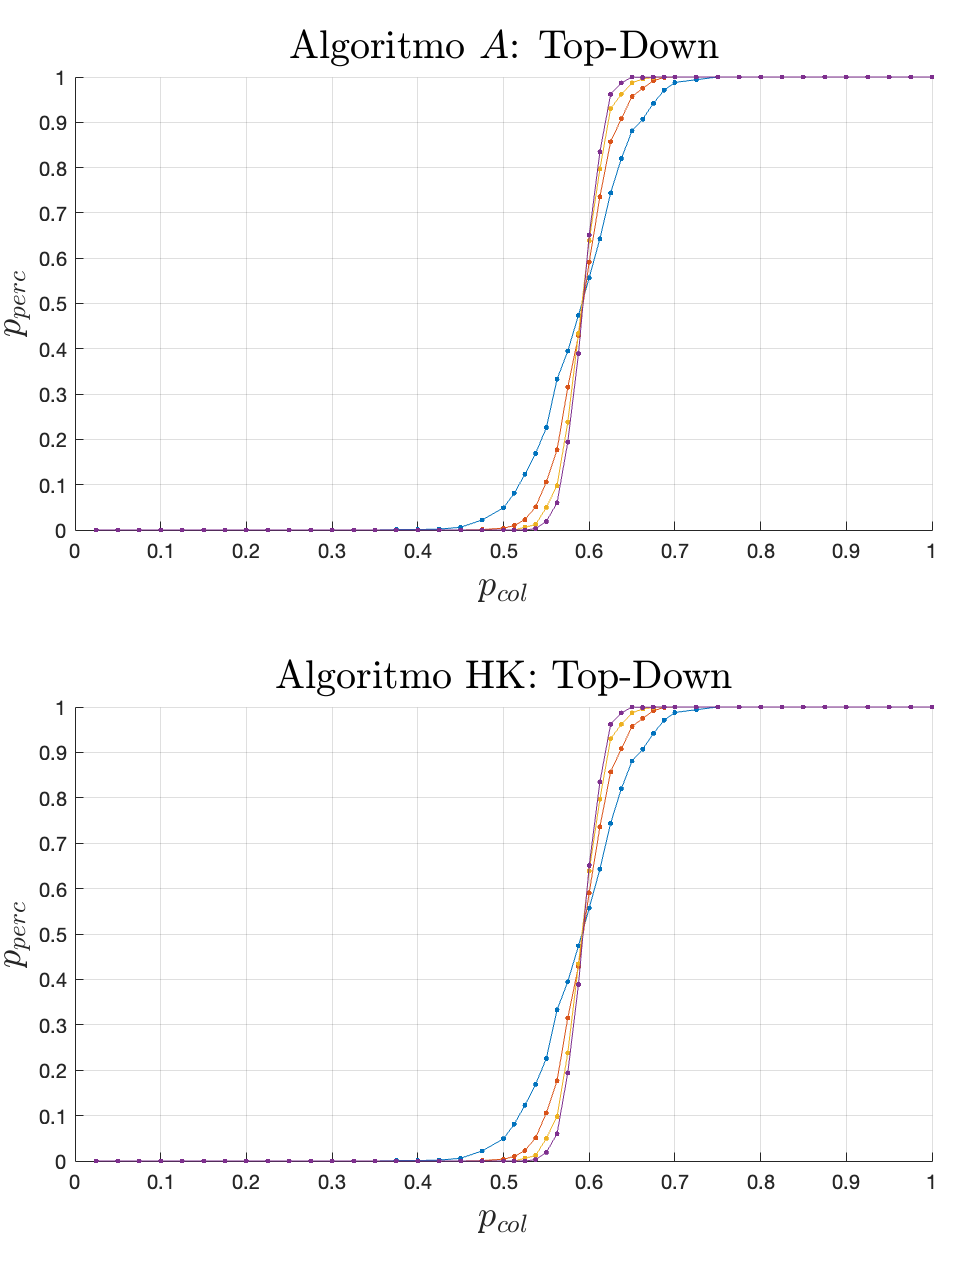
\includegraphics[width=0.9\columnwidth]{compare_threshold_1.png}
    \caption{Confronto tra le frequenze di percolazione top-bottom ottenute nell'esecuzione
    dei due algoritmi.}
    \label{fig:compare_threshold}
\end{figure}
Risulta interessante eseguire un confronto con la Fig. \ref{fig:threshold} 
relativa al reticolo di taglia infinita: per dimensioni del reticolo più grandi, ci 
si avvicina infatti al suddetto grafico.
Un'altra caratteristica importante da verificare è che le frequenze di 
percolazione top-bottom registrate coincidano con quelle left-right, nel limite 
dell'errore commesso. Le modalità di svolgimento sono le stesse, con l'aggiunta 
delle misurazioni dell'errore, calcolato come radice quadrata della quantità 
$D_{f_{perc}}$ descritta nell'Eq. \ref{eq:d_f_perc}.
Nel grafico in Fig. \ref{fig:th_errors} viene mostrato un confronto tra i valori 
ottenuti nei due casi con l'algoritmo HK. Ciò che balza all'occhio è la 
superiorità degli errori intorno a $0.6$, valore attorno al quale 
si osserva una crescita piuttosto rapida della frequenza di percolazione.
Si compone di tre iterazioni: una per variare la 
taglia del reticolo, una per variare la probabilità di occupazione e un'ultima per 
eseguire un numero sufficiente di esperimenti affinché i risultati siano significativi.
Le frequenze dei due algoritmi sono calcolate con metodi diversi ma equivalenti:
nel primo caso si ``conta'' quante volte la variabile caratteristica ha assunto valore 1
e si divide il totale per il numero di esperimenti $N$; nel secondo caso si utilizza la 
funzione built-in di Matlab \texttt{mean(x)}, che svolge gli stessi passaggi.
Il Cod. \ref{cod:compare} mostra le istruzioni in Matlab per calcolare le quantità 
mostrate nei due grafici. Si è omessa l'implementazione in codice Matlab delle funzioni 
\texttt{CercaCluster3} e \texttt{CercaClusterHK}, del tutto analoghe all'implementazione 
mostrata tramite pseudocodice negli Alg. \ref{alg:standard} e \ref{alg:HK}. \\


\begin{figure}[ht]
    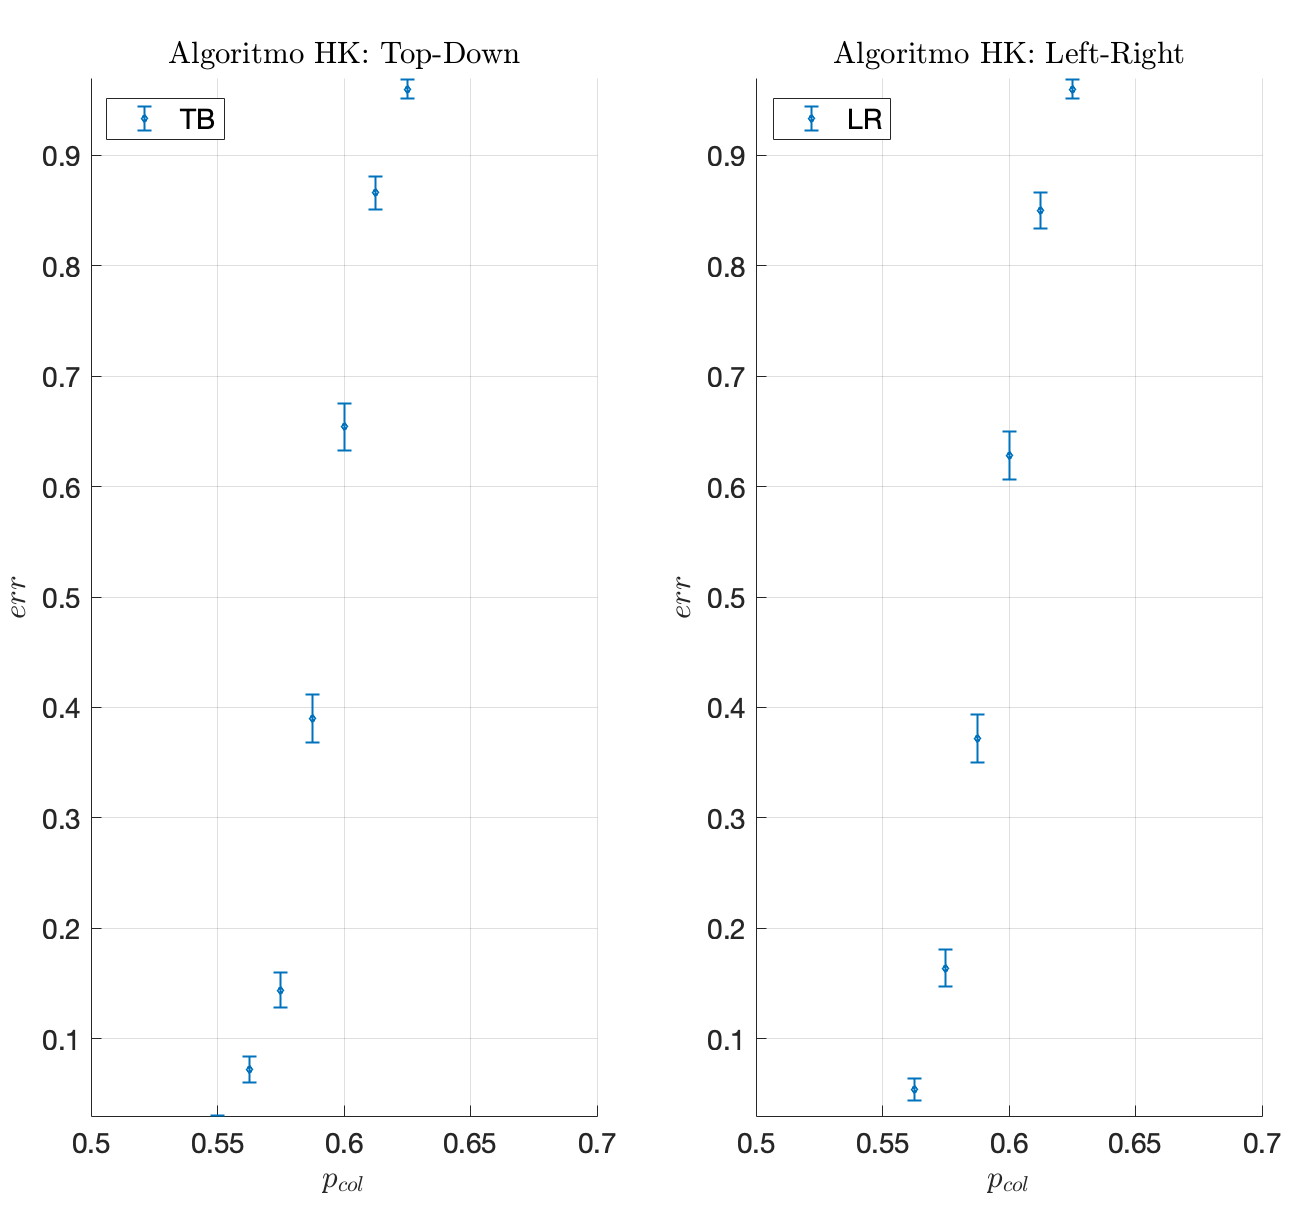
\includegraphics[width=\columnwidth]{errors.png}
    \caption{Confronto tra le frequenze di percolazione top-bottom e left-right,
    con rispettivi errori.}
    \label{fig:th_errors}
\end{figure}
\begin{lstlisting}[caption={Porzione di codice relativa al confronto tra algoritmi e 
    alla frequenza di percolazione top-bottom e left-right.}, label={cod:compare}]
for ij = 1:length(L)
    for ii = 1:length(p)
        pp = p(ii);
        s3TB = 0;
        s3LR = 0;
        sHKTB = 0;
        sHKLR = 0;
        espTB = zeros(N,1);
        espLR = zeros(N,1);
        for j = 1:N
            ret = rand(L(ij))<pp;
            res3 = CercaCluster3(ret);
            resHK = CercaClusterHK(ret);
            s3TB = s3TB + res3.percolazioneTB;
            s3LR = s3LR + res3.percolazioneLR;
            espTB(j) = resHK.percolazioneTB;
            espLR(j) = resHK.percolazioneLR;
        end
        probPercTB3(ij,ii) = s3TB / N;
        probPercLR3(ij,ii) = s3LR / N;
        probPercTBHK(ij,ii) = mean(espTB);
        probPercLRHK(ij,ii) = mean(espLR);
        erroreTB(ij,ii) = std(espTB) / sqrt(N);
        erroreLR(ij,ii) = std(espLR) / sqrt(N);
    end
end
\end{lstlisting}

\subsection*{Calcolo delle osservabili}
Lo stesso procedimento necessario per calcolare la frequenza di percolazione è stato svolto per 
le altre osservabili. In Fig. \ref{fig:distributions} si possono riscontrare i comportamenti 
attesi, descritti nella sezione precedente.
Anche in questo caso, viene acclusa l'implementazione in Matlab nel Cod. \ref{cod:distributions}.
Insieme alle quantità, vengono calcolati anche i rispettivi errori, con tecniche analoghe a quanto visto 
fin ora. Per queste quantità valgono infatti le stesse considerazioni fatte sulla natura di $f_{perc}$,
legate alla validità della media e varianza garantita per mezzo di 
TLC e Legge dei Grandi Numeri.
\begin{figure}[ht]
    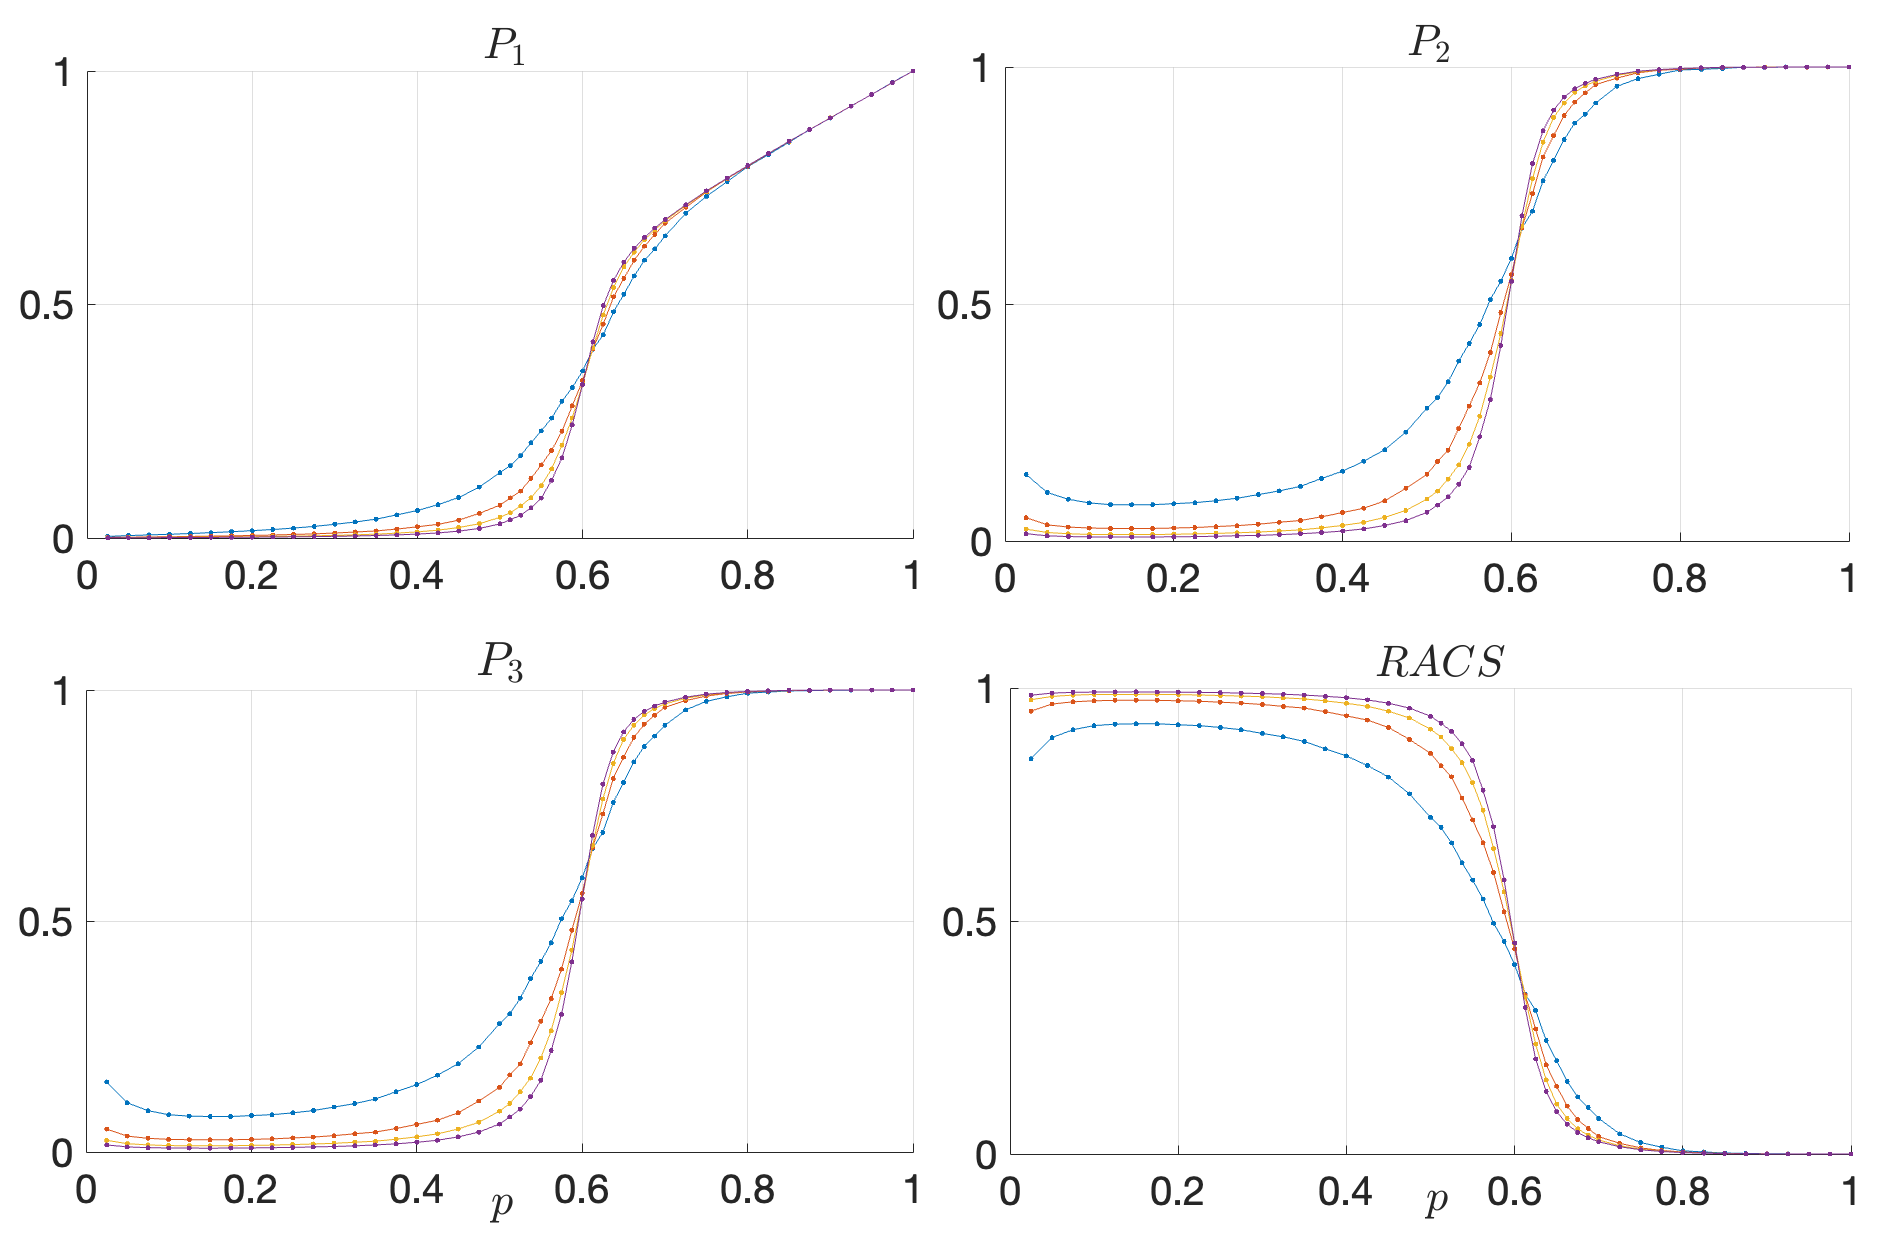
\includegraphics[width=\columnwidth]{p1p2p3racs_3.png}
    \caption{Distribuzioni delle osservabili calcolate in $N=1000$ esperimenti al variare dei parametri.}
    \label{fig:distributions}
\end{figure}
\begin{lstlisting}[caption={Porzione di codice per il calcolo delle osservabili.},label={cod:distributions}]
for ij = 1:length(L)
    for ii = 1:length(p)
        pp = p(ii);
        for j = 1:N
            ret = rand(L(ij))<pp;
            resHK = CercaClusterHK(ret);

            MYsz(ij,j,ii) = mean(resHK.cluSz);
            MYmaxSz(ij,j,ii) = max(resHK.cluSz);
            MYnumCLU(ij,j,ii) = length(resHK.cluSz);
            MYnumCol(ij,j,ii) = sum(resHK.cluSz);
        end
    end
   
    sMax=squeeze(MYmaxSz(ij,:,:));
    P1=sMax./L(ij)^2;
    errore1=std(P1)./sqrt(length(P1));
    P1=mean(P1);

    P2=sMax./(p*L(ij)^2);
    errore2=std(P2)./sqrt(length(P2));
    P2=mean(P2);

    occupied=squeeze(MYnumCol(ij,:,:));
    P3=sMax./occupied;
    P3=squeeze(P3);
    errore3=std(P3)./sqrt(size(P3,2));
    P3=mean(P3);

    occupiedReduced = squeeze(MYnumCol(ij,:,:)-MYmaxSz(ij,:,:));
    racs=occupiedReduced./occupied;
    erroreRacs=std(racs)/sqrt(length(racs));
    racs=mean(racs);
end
\end{lstlisting}

Per completezza, si aggiunge anche il grafico in Fig. \ref{fig:dist_errors} che confronta i vari errori 
ottenuti nel calcolo di ciascuna. Occorre prestare attenzione alla scala
sugli assi dei grafici: per questioni pratiche di visualizzazione, si è preferito
avere risultati più chiari, ma su scale leggermente diverse.
\begin{figure}[ht]
    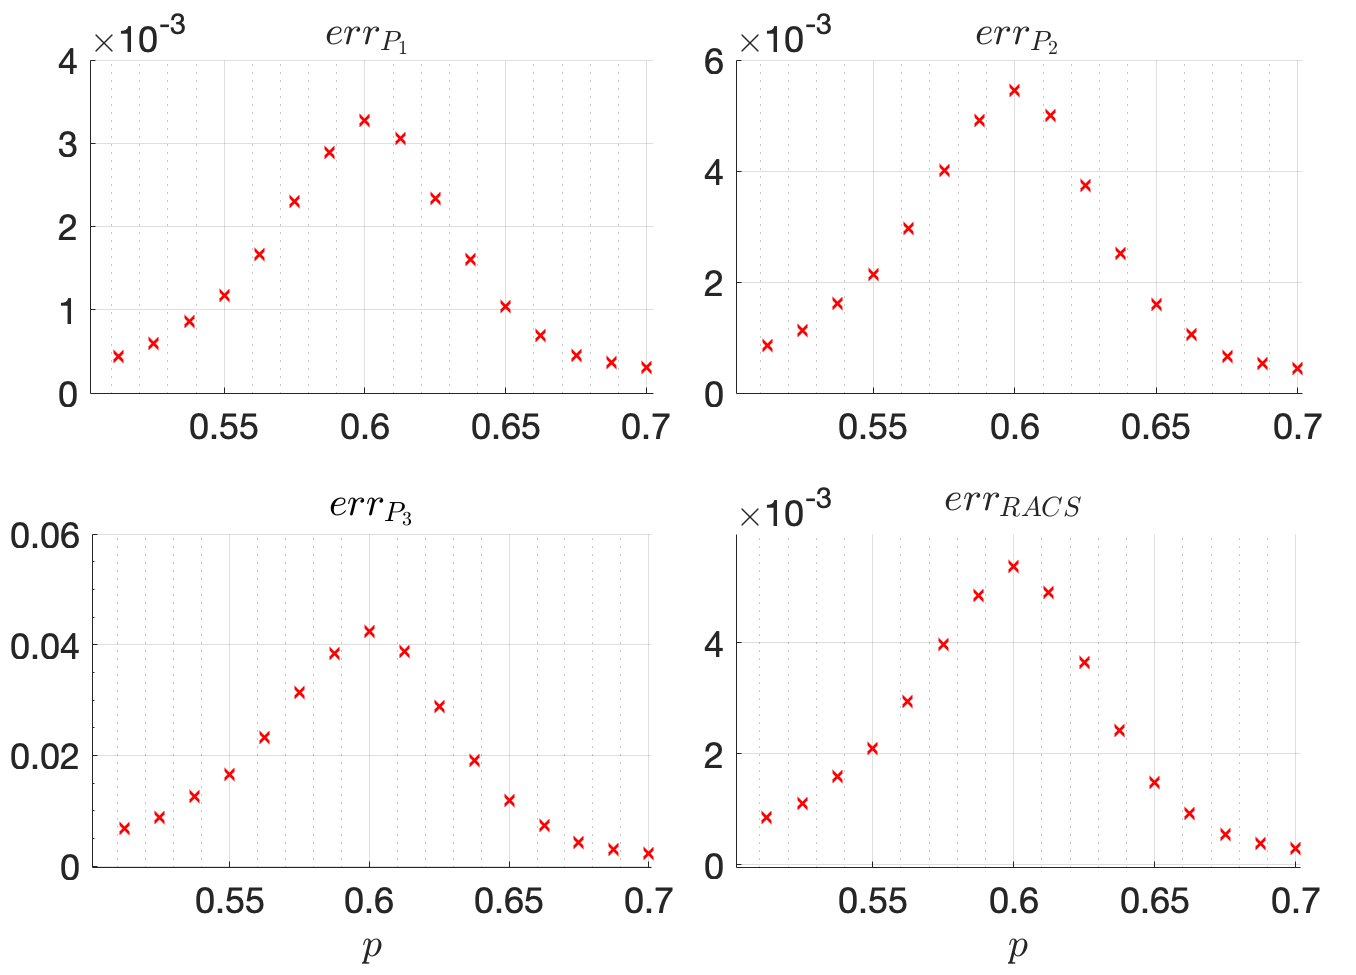
\includegraphics[width=\columnwidth]{dist_errors.png}
    \caption{Errori ottenuti nel calcolo delle osservabili.}
    \label{fig:dist_errors}
\end{figure}

\subsection*{Tempi di esecuzione}
Come ultimo risultato verranno discussi i tempi di esecuzione di ciascun algoritmo.
Prima di farlo, però, occorre precisare che Matlab non è l'ambiente di sviluppo migliore per valutare 
differenze di costo computazionale, a causa dei seguenti svantaggi (almeno per questo caso) che lo costituiscono:
\begin{itemize}
    \item operazioni matriciali: Matlab opera su strutture dati che rappresentano matrici,
        non è quindi ottimizzato per esecuzioni di tipo iterativo;
    \item ricorsione: le strutture dati utilizzate per 
        rappresentare il controllo di flusso non sempre sono adatte a sostenere lo spazio 
        richiesto da chiamate ricorsive;
    \item ``tic toc'': è il metodo per misurare i tempi di esecuzionein Matlab; non ha un buon funzionamento 
        in caso di quantità elevate di prove ripetute, soprattutto se molto vicine tra loro.
\end{itemize}
In fondo, Matlab rimane un linguaggio relativamente di alto livello rispetto 
ad alcune sue controparti come C++ per \texttt{opencv}.
Esistono alcune funzionalità che permettono di generare codice C++ o per GPU, ma non verranno affrontate in questa relazione.
Va comunque ricordato che Matlab ha molti altri pregi, tra cui la flessibilità
per la creazione di modelli, caratteristica fondamentale per il progetto.
Per tutte queste ragioni, i due algoritmi sono stati confrontati solo sulla parte 
relativa al cluster-finding. Il motivo dietro a questo è che nell'algoritmo Hoshen-Kopelman sono 
necessarie chiamate ricorsive per capire se due siti appartengono allo stesso cluster, e questa 
proprietà va verificata per tutti i siti dei bordi, causando un \textit{overhead}.
\begin{figure}[ht]
    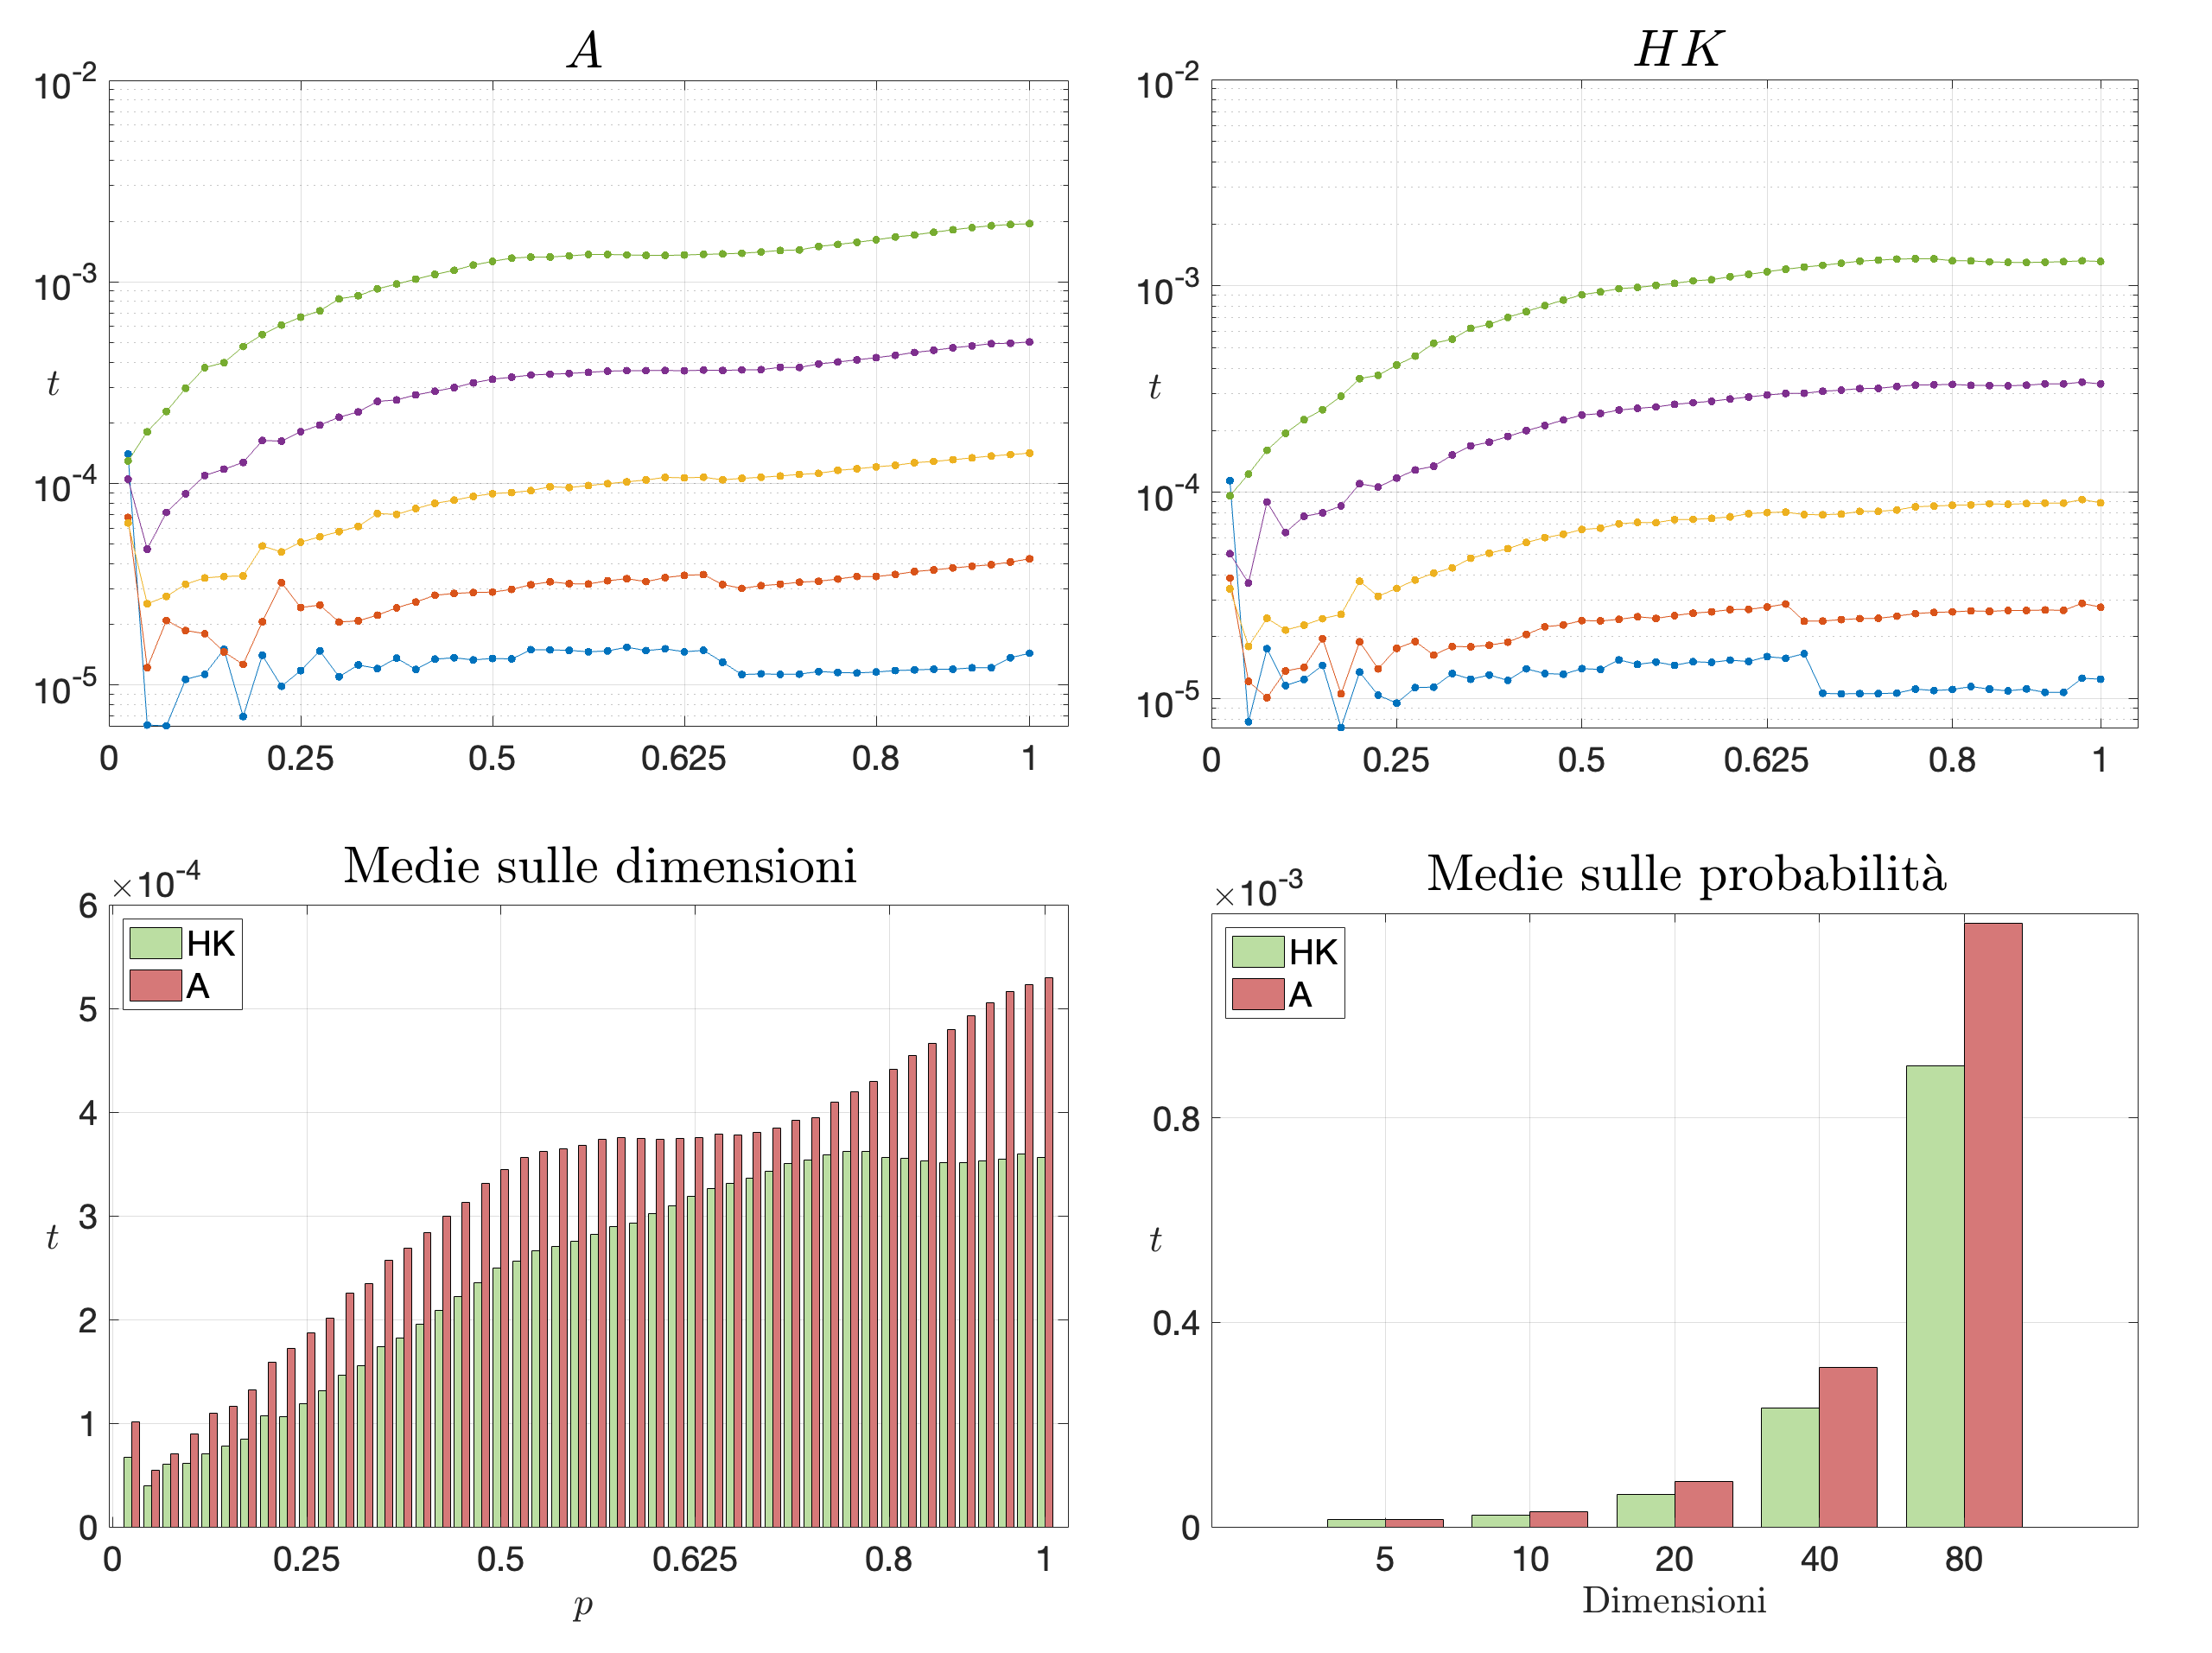
\includegraphics[width=\columnwidth]{times.png}
    \caption{Confronto dei tempi di esecuzione dei due algoritmi.}
    \label{fig:times}
\end{figure}

In Fig. \ref{fig:times} sono presenti 4 grafici che mostrano un confronto sugli andamenti dei 
tempi di esecuzione calcolati nelle due casistiche.
Anche in questo caso, la statistica viene fatta fissando i parametri (dimensione e probabilità di occupazione),
per poi effettuare un numero $N$ arbitrariamente grande di esperimenti.
Viene quindi eseguito prima $N$ volte l'algoritmo $A$, registrando il tempo impiegato e dividendolo per $N$
(si ottiene quindi una media per l'esecuzione singola).
Lo stesso viene fatto per l'algoritmo $HK$. Ciò che si ottiene sono due matrici $|P| \times |D|$, 
dove $D=[5 \; 10 \; 20 \; 30 \; 40]$ è l'array delle dimensioni e $P$ è l'array delle probabilità di 
occupazione.

I primi due grafici rappresentano proprio le due matrici ottenute, dove gli assi $y$ sono in scala 
logaritmica per avere un confronto visivo migliore. I colori indicano le diverse dimensioni dei reticoli 
negli esperimenti. Anche se di poco, in generale si notano tempi minori nell'algoritmo $HK$.
Nel terzo grafico viene fatta una media sulle dimensioni, in modo che rimangano solo due serie di dati da confrontare.
In pratica, si può pensare alle quantità mostrate nel terzo grafico come ``medie'' di quelle mostrate nei primi due.
Nell'ultimo caso, invece, la media viene fatta sulle probabilità e la lunghezza delle due serie di dati da confrontare è 
di 5 elementi, come il numero elementi nell'array delle dimensioni. 
Anche in questo caso, le tempistiche di $HK$ sono minori rispetto ad $A$, come 
si aveva ragione di credere.